\documentclass[10pt]{beamer}
% \usepackage[colorlinks=true,citecolor=blue, linkcolor=blue]{hyperref}
\usepackage{hyperref}
\usepackage[utf8x]{inputenc}
\usepackage{algorithm, algorithmic}
\usepackage[ruled,vlined]{algorithm2e}
% \usepackage{fontawesome}
\usepackage{graphicx}
% \usepackage[english]{babel}
\usepackage[nodayofweek]{datetime}

\usepackage[colorinlistoftodos]{todonotes}
\usepackage{graphicx}
\usepackage{mathtools}
\usepackage{amssymb}
\usepackage{amsmath}
\usepackage{bbm}
\usepackage{pdflscape}
\usepackage{caption}
\usepackage{subcaption}
\usepackage[T1]{fontenc}
% \usepackage[utf8]{inputenc}
\usepackage{authblk}
\usepackage{pdfpages}
\usepackage{setspace} 
\usepackage{booktabs}
\usepackage{longtable}
\usepackage{float}
\usepackage{tikz}
% \usepackage{multirow}
% \setlength{\tabcolsep}{5pt}
% \usepackage[parfill]{parskip}
% \renewcommand{\arraystretch}{1.5}

% ------------------------------------------------------------------------------
% Use the beautiful metropolis beamer template
% ------------------------------------------------------------------------------
\usepackage[T1]{fontenc}
\usepackage{fontawesome}
\usepackage{FiraSans} 
\mode<presentation>
{
  \usetheme[progressbar=foot,numbering=fraction,background=light]{metropolis} 
  \usecolortheme{default} % or try albatross, beaver, crane, ...
  \usefonttheme{default}  % or try serif, structurebold, ...
  \setbeamertemplate{navigation symbols}{}
  % \setbeamertemplate{caption}[numbered]
  %\setbeamertemplate{frame footer}{My custom footer}
} 

\setbeamertemplate{section in toc}{\hspace*{1em}\inserttocsectionnumber.~\inserttocsection\par}
\setbeamertemplate{subsection in toc}{\hspace*{2em}\inserttocsectionnumber.\inserttocsubsectionnumber.~\inserttocsubsection\par}

% ------------------------------------------------------------------------------
% beamer doesn't have texttt defined, but I usually want it anyway
% ------------------------------------------------------------------------------
\let\textttorig\texttt
\renewcommand<>{\texttt}[1]{%
  \only#2{\textttorig{#1}}%
}

% ------------------------------------------------------------------------------
% minted
% ------------------------------------------------------------------------------
\usepackage{minted}


% ------------------------------------------------------------------------------
% tcolorbox / tcblisting
% ------------------------------------------------------------------------------
\usepackage{xcolor}
\definecolor{codecolor}{HTML}{FFC300}

\usepackage{tcolorbox}
\tcbuselibrary{most,listingsutf8,minted}

\tcbset{tcbox width=auto,left=1mm,top=1mm,bottom=1mm,
right=1mm,boxsep=1mm,middle=1pt}

\newtcblisting{myr}[1]{colback=codecolor!5,colframe=codecolor!80!black,listing only, 
minted options={numbers=left, style=tcblatex,fontsize=\tiny,breaklines,autogobble,linenos,numbersep=3mm},
left=5mm,enhanced,
title=#1, fonttitle=\bfseries,
listing engine=minted,minted language=r}


% ------------------------------------------------------------------------------
% Listings
% ------------------------------------------------------------------------------
\definecolor{mygreen}{HTML}{37980D}
\definecolor{myblue}{HTML}{0D089F}
\definecolor{myred}{HTML}{98290D}

\usepackage{listings}

% the following is optional to configure custom highlighting
\lstdefinelanguage{XML}
{
  morestring=[b]",
  morecomment=[s]{<!--}{-->},
  morestring=[s]{>}{<},
  morekeywords={ref,xmlns,version,type,canonicalRef,metr,real,target}% list your attributes here
}

\lstdefinestyle{myxml}{
language=XML,
showspaces=false,
showtabs=false,
basicstyle=\ttfamily,
columns=fullflexible,
breaklines=true,
showstringspaces=false,
breakatwhitespace=true,
escapeinside={(*@}{@*)},
basicstyle=\color{mygreen}\ttfamily,%\footnotesize,
stringstyle=\color{myred},
commentstyle=\color{myblue}\upshape,
keywordstyle=\color{myblue}\bfseries,
}

% ------------------------------------------------------------------------------
% The Document
% ------------------------------------------------------------------------------

\begin{document}

\title{Developing clustering algorithms for conditional extremes models}

\date{
  \footnotesize Thesis formulation report (TFR) presentation \\ 
  \today \\
  % \shortdate \\
  \vspace{0.4cm}
  \emph{Paddy O'Toole, supervised by Christian Rohrbeck}
}

% \title{Wessex Water: Bayesian Network for Source Apportionment}
% \author{\emph{Sam Williams, Paddy O'Toole, Christian Rohrbeck, Haiyan Zheng, Emiko Dupont}}
% \date{\today}


\frame{\titlepage}

%==================================================

% \frame{\begin{small}
% \frametitle{Overview}
% \tableofcontents\end{small}}

%=================================================
\begin{frame}
\frametitle{Table of Contents}
\tableofcontents
\end{frame}

\section{Introduction}

% TODO: Perhaps add one more introduction slide?

% Motivation behind EVT
\begin{frame}{Introduction}
% \todo{Include use cases}
    % \begin{itemize}
    %     \item Extreme Value Theory is a field of statistics concerned with modelling the extremal tail of distributions, where standard methods do not perform well
    %     \item Many use cases, particularly popular for environmental data (rainfall, flooding, storms, temperature), where tail events often catastrophic. 
    %     \item Concerned with performing \textbf{extremal clustering}, helps with dimensionality reduction and understanding patterns in data
    %     % Need to have metric for magnitude over which to deem events as extreme, and then frequency or concommitant extremes for clustering 
    % \end{itemize}

   \begin{minipage}{0.49\textwidth}
        % Anything else to add here?
        \begin{itemize}
            \item Extreme Value Theory models the extreme tails of distributions % standard models don't work well
            \item Only known method that can reliably predict beyond observations in extremal context
            \item Applications include in finance and insurance, and environmental data, such as extreme precipitation and/or wind speeds. % todo: Rewrite this!
        \end{itemize}
   \end{minipage}
   \hfill
   \begin{minipage}{0.49\textwidth}
     % \centering
     \vspace{}
     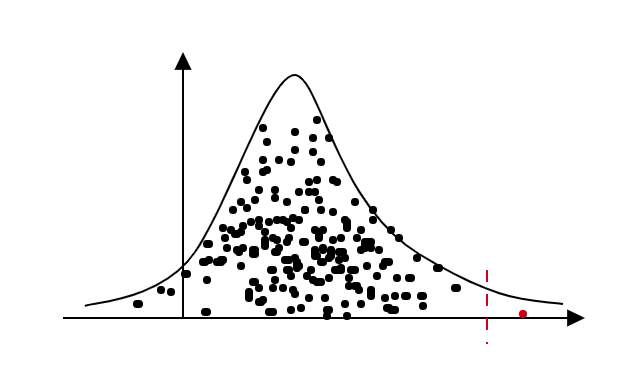
\includegraphics[width=6cm]{latex/images/tail.png}
   \end{minipage}
\end{frame}

% Images of Pulteney Bridge Weir and plaque
\begin{frame}
   \begin{minipage}{0.49\textwidth}
     \vspace{}
     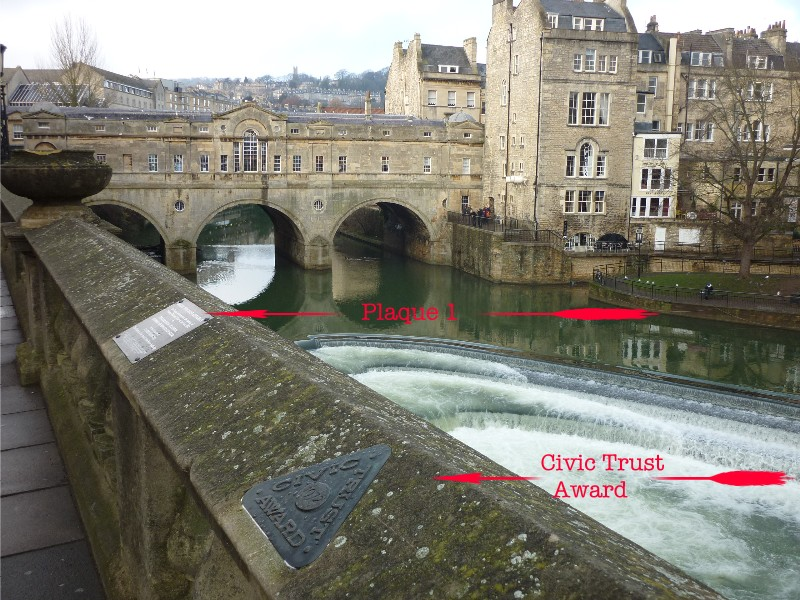
\includegraphics[width=6cm]{latex/images/civictrustaward_location.jpg}
   \end{minipage}
   \hfill
   \begin{minipage}{0.49\textwidth}
   % todo: Rotate image (and add in!)
   \end{minipage}
\end{frame}

% MV extremes, uses, methods, shortcomings - clustering
\begin{frame}{Multivariate extremes}
    \begin{itemize}
        \item Often, for a 
    \end{itemize}
\end{frame}

\section{Motivating example}

% Describe motivating example
\begin{frame}{Motivating example - Ireland}

   \begin{minipage}{0.49\textwidth}
   \end{minipage}
   \begin{minipage}{0.49\textwidth}
     \vspace{}
     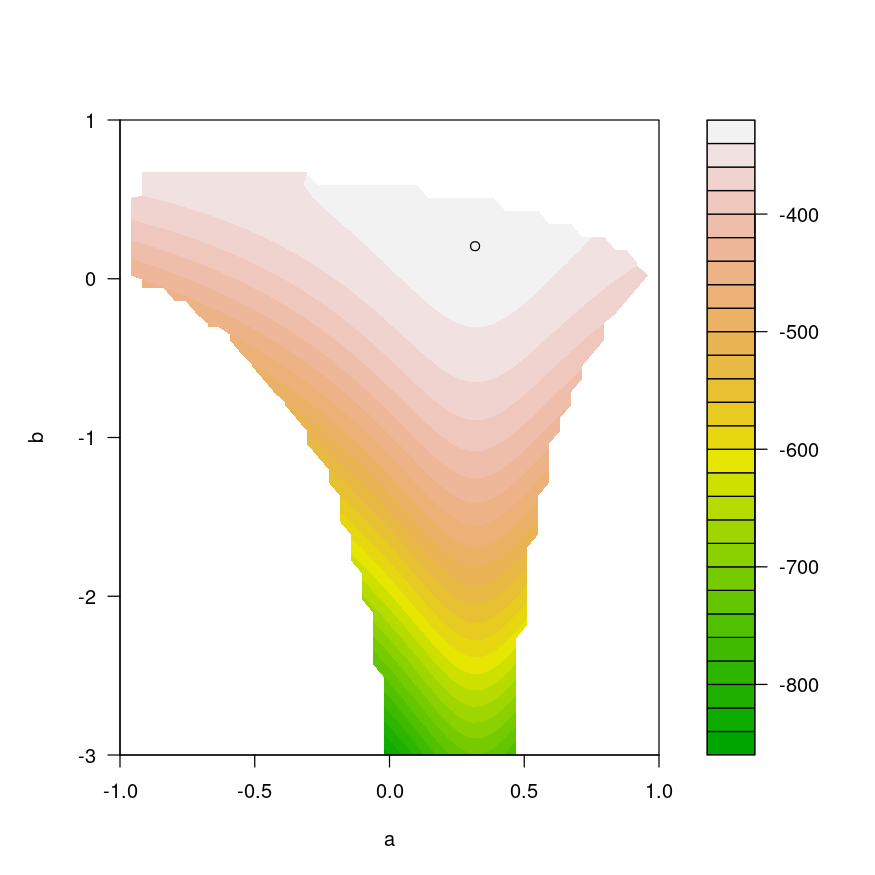
\includegraphics[width=6cm]{latex/plots/Rplot.png}
   \end{minipage}

\end{frame}

\section{Univariate extremes}


% GPD formula, threshold selection, non-stationary version
\begin{frame}{Generalised Pareto distribution}
\end{frame}

% Plot of sigma, xi values across Ireland
\begin{frame}{Motivating example}

\end{frame}

\section{Conditional extremes}
\begin{frame}{Introduction}

\end{frame}

% Univariate piecewise function
\begin{frame}{Univariate}

\end{frame}

% Transform to Laplace
\begin{frame}{Marginal transformation}
\end{frame}

% Multivariate piecewise function, Z, Y independent
\begin{frame}{Multivariate}

\end{frame}

% Methods for estimation, assumption on Z
\begin{frame}{Estimation}

\end{frame}

% Poor results initially, high uncertainty
\begin{frame}{Motivating example - Sensitivity}

\end{frame}

% Improved here
\begin{frame}{Fixing $\beta$}

\end{frame}

% Map of alpha values
\begin{frame}{Results}

\end{frame}

% Rain vs wind speed alpha vals, and vs lon/lat
\begin{frame}{Interpretation}

\end{frame}

% Briefly talk about extensions to model
\begin{frame}{Extensions to CE model}

\end{frame}

% TODO: May need more information/slides here
\section{Clustering}

% Reasons for and types of clustering 
\begin{frame}{Clustering}
\end{frame}

\begin{frame}{Explanatory clustering}
\end{frame}

\begin{frame}{Hierarchical clustering}
\end{frame}

\section{Conclusions and future work}

\begin{frame}{Conclusions}
\end{frame}

\begin{frame}{Future work}
\end{frame}

% TODO: Add references!

%============================================================
% \frame{
% \vskip30mm
% \centerline{\Large\color{violet}\textsc{Thank you!}}
% \centerline{\Large\color{violet}\textsc{Any Questions?}}
% \vskip40mm
% }





\end{document}
